\setlength{\textheight}{\textheight+\footskip}
\newpage
\setlength{\footskip}{0pt}

\section*{Supplementary material}

\begin{figure}[h!] 
    \begin{adjustwidth}{-20mm}{-10mm}
    \centering 
    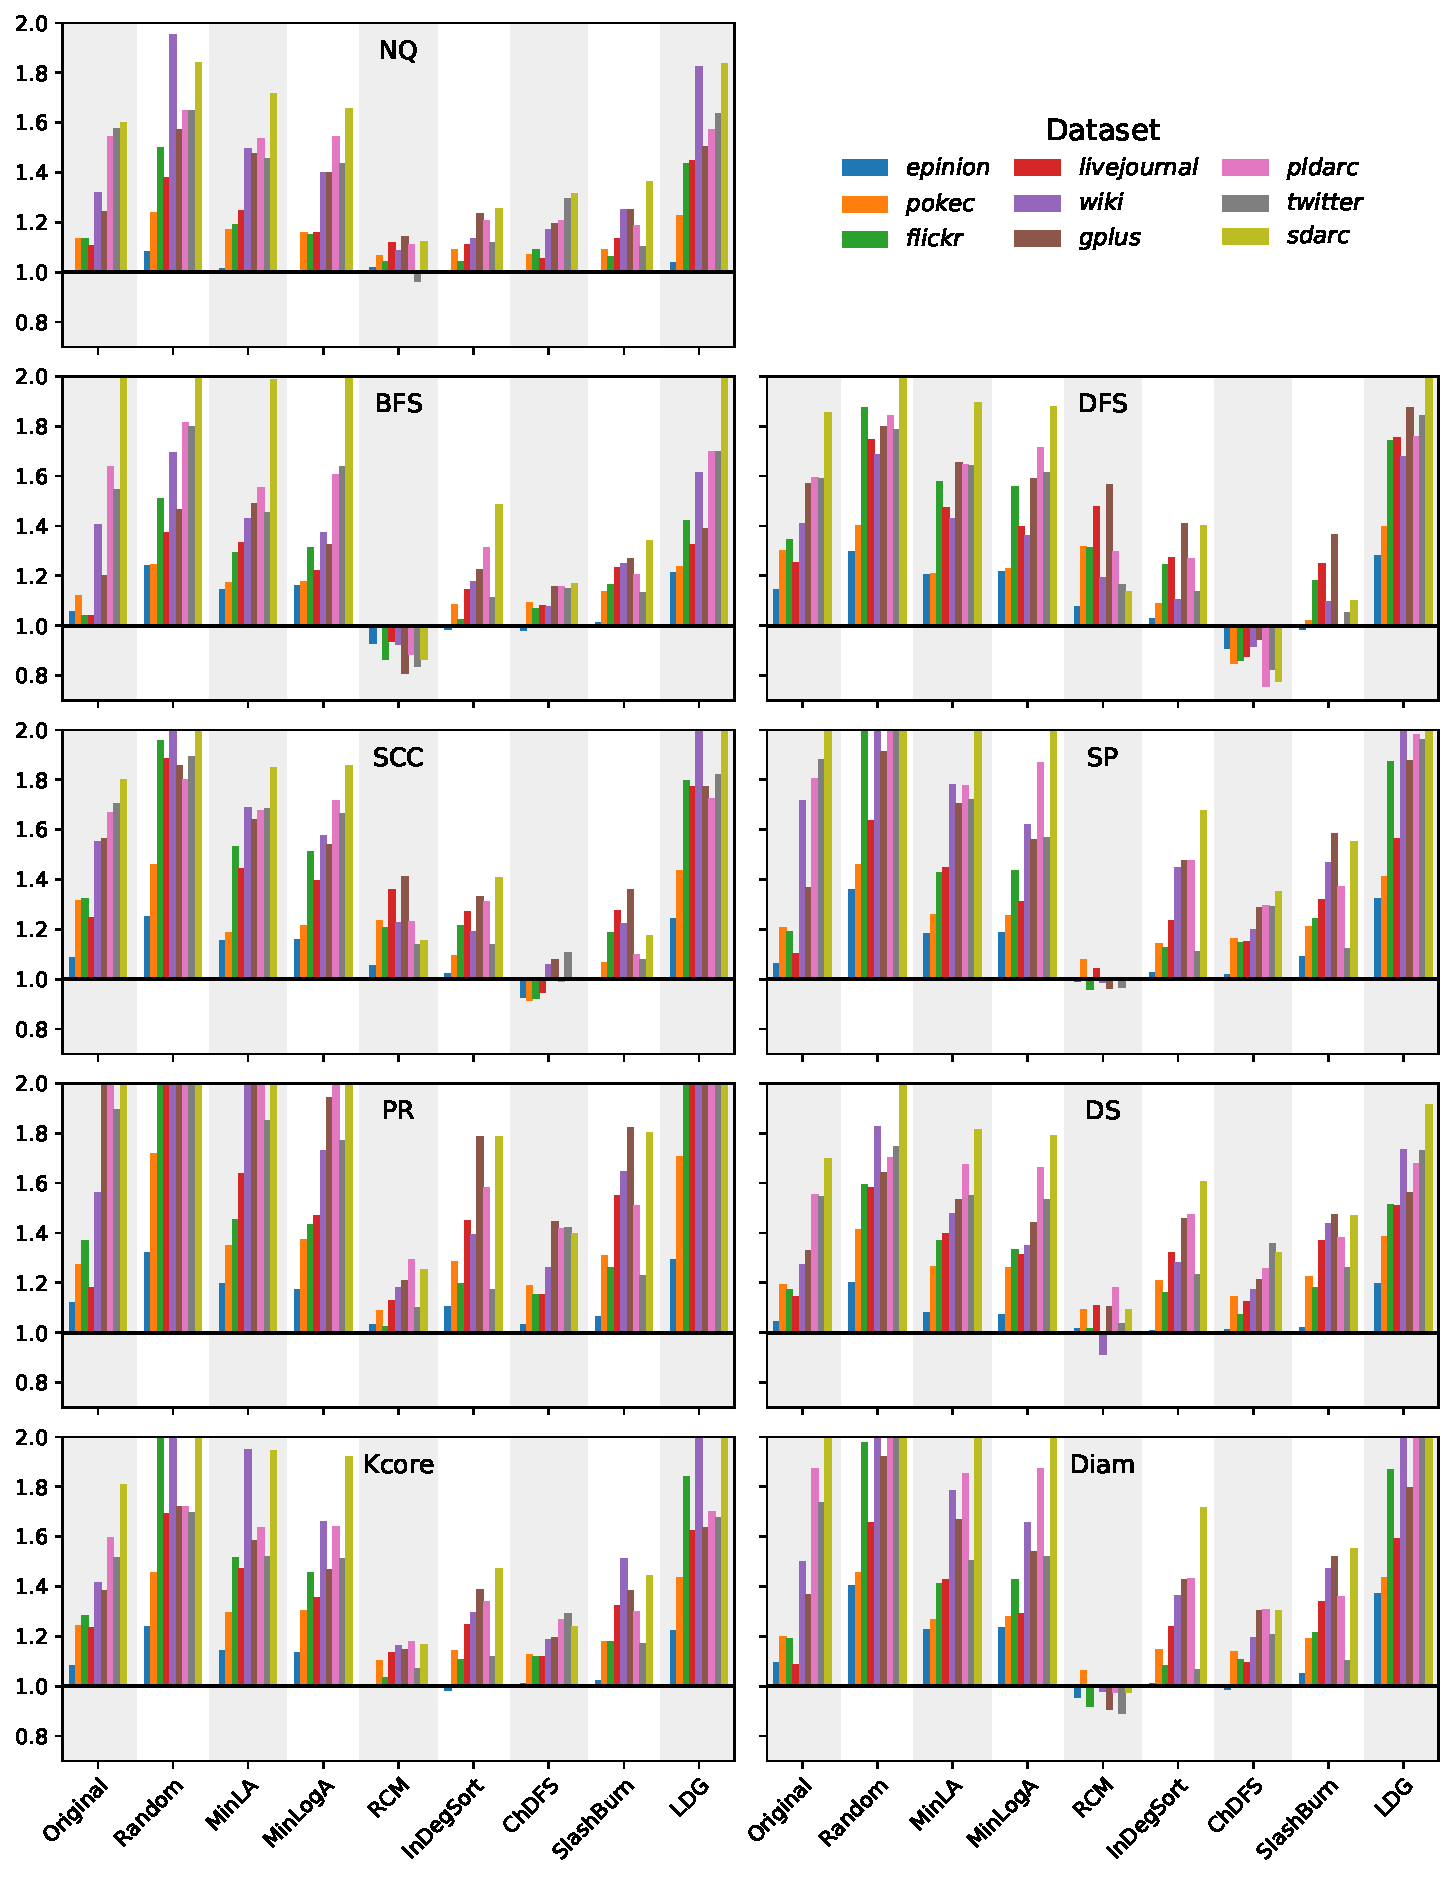
\includegraphics[width=\linewidth]{img/img-speedup-grouped.pdf}
    \caption{\textbf{Speedup of Gorder grouped by ordering.} For each algorithm and each ordering, bars represent the relative duration on each dataset compared to Gorder, taken as a reference. For readability, the y-axis is cut above factor~2. This figure displays the same information as Figure~\ref{img-speedup} but groups bars by ordering instead of dataset.}\label{img-speedup-grouped}
    \end{adjustwidth}
\end{figure}

